\documentclass[accentcolor=tud1b,colorbacktitle]{tudbeamer}
\usepackage{graphicx,amsmath,bm,color,psfrag}

%\definecolor{TUDgreen}{rgb}{0.4980,0.6706,0.0863} % (127,171,22)
\definecolor{TUDblue}{rgb}{0,0.3529,0.6627}       % (0,90,169)
%\definecolor{TUDred}{rgb}{0.9020,0,0.1020}        % (230,0,26)


\title{Maximum-Likelihood Detection in\\ DWT Domain Image Watermarking\\ using Laplacian Modeling}
\subtitle{by T. M. Ng and H. K. Garg}

\date{\today}
\author[V.Mees \and M.Stiefel]{Valentin Mees \and Max Stiefel}               % <--- your name here!
\logo{\textcolor{TUDblue}{\large SPG}}
\institute[SPG]{}


\AtBeginSection[]{%
  \frame<beamer>{ 
    \frametitle{Outline}   
    \tableofcontents[currentsection]}
}%

\begin{document}

\begin{titleframe}
\centering
\vfill
\textit{\Large \insertauthor}
\vfill

\includegraphics[width=0.2\textwidth]{figures/spg_logo}
\vfill
   Signal Processing Group\\
   Institute of Telecommunications\\
   Technische Universit\"at Darmstadt\\
\end{titleframe}
%

\frame<beamer>{\frametitle{Outline} \tableofcontents}

%\section*{Motivation}
%\begin{frame}\frametitle{\insertsection}
\begin{block}{Imperceptible digital watermarks}
\begin{itemize}
\item invisible to the human eye
\item can disclose copyright infringements
\end{itemize}
\end{block}

\begin{block}{in Discrete Wavelet domain}
\begin{itemize}
\item robust to modification in spatial domain
\end{itemize}
\end{block}

\begin{block}{using stochastic detection}
\begin{itemize}
\item Neyman-Pearson Test yields optimal detection probability for given false alarm rate
\end{itemize}
\end{block}

\end{frame}

%\section{DWT watermarking}
%\begin{frame}{\insertsection}{Original proposal by Kim, Kwon and Park}
	\begin{columns}[T]
	\column{0.5\textwidth}
	\begin{itemize}
	\item three-level pyramid decomposition
	\item watermark embedding in all sub-bands except $LH_1$, $HL_1$, $HH_1$
	\newline \textcolor{TUDblue}{$\Rightarrow$} low energy in those bands
	\item multi-resolution for robustness
	\item embedding strength proportional to band energy
	\end{itemize}
	\column{0.5\textwidth}
	\centering
	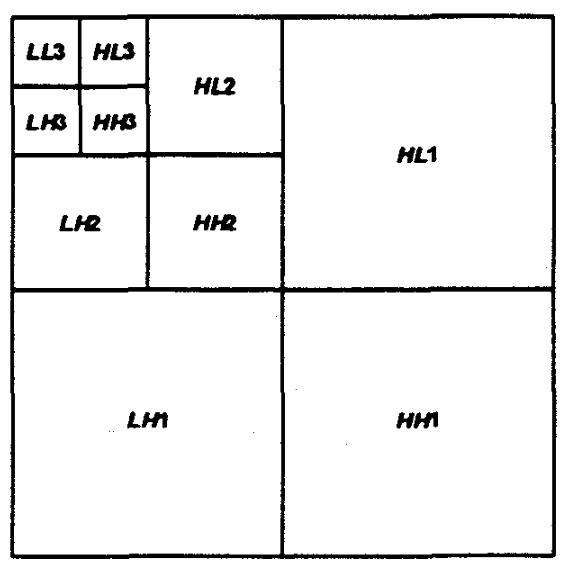
\includegraphics[width=.8\textwidth]{Bilder/threelayerMotivation} 
	
	DWT decomposition (\cite{779947})
	\end{columns} 	
\end{frame}

\begin{frame}{\insertsection}{Implemented method}
	\begin{columns}[T]
	\column{0.5\textwidth}
	\begin{itemize}
	\item Daubechies filter used for DWT
	\item three-level pyramid decomposition
	\item watermark embedding in high resolution sub-bands $LH_3$, $HL_3$, $HH_3$ 
	\item embedding strength $\alpha_i$
	\newline \textcolor{TUDblue}{$\Rightarrow$} robustness vs. imperceptibility %chosen that $\text{PSNR} = \SI{45}{\deci\bel}$
	\item each sub-band $B$ has $N_B = 4096$ coefficients 
	\newline \textcolor{TUDblue}{$\Rightarrow$} watermark size $N = 12288$
	\item multiplicative embedding	
	\newline \textcolor{TUDblue}{$\Rightarrow$} $y_i = x_i(1+\alpha_iw_i)$
	\end{itemize}
	\column{0.5\textwidth}
	\centering
	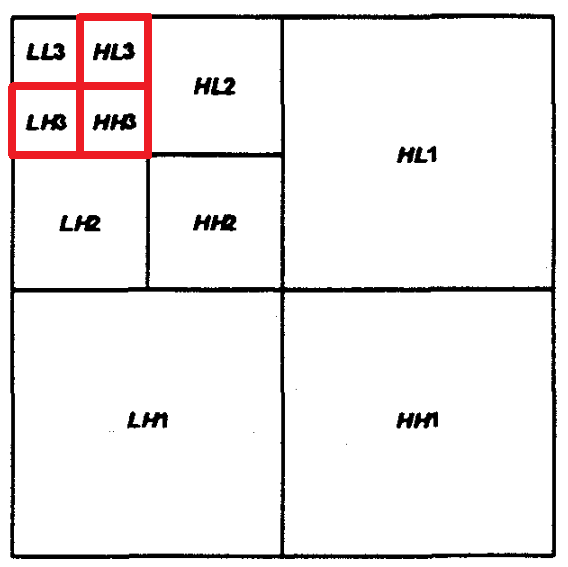
\includegraphics[width=.8\textwidth]{Bilder/threelayerMotivationPainted} 
	
	DWT decomposition with used sub-bands 
	\end{columns} 	
\end{frame}

\begin{frame}{\insertsection}{Implemented method}
	\begin{columns}[T]
	\column{0.5\textwidth}
	\begin{itemize}
	\item each sub-band $B$ has $N_B = 4096$ coefficients 
	\newline \textcolor{TUDblue}{$\Rightarrow$} watermark size $N = 12288$
	\item Watermarks are i.i.d. $\mathcal{U}(-1, 1)$
	\item Original sub-bands i.i.d., assumed to be Laplacian distributed
	\item No correlation between sub-bands assumed
	\end{itemize}
	\column{0.5\textwidth}
	\centering
	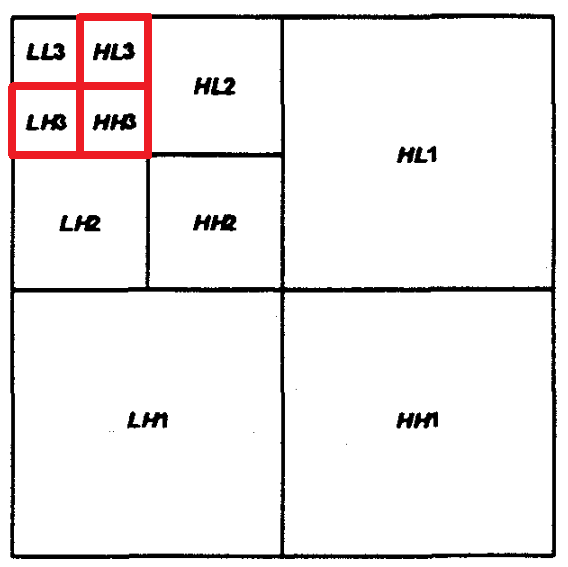
\includegraphics[width=.8\textwidth]{Bilder/threelayerMotivationPainted} 
	
	DWT decomposition with used sub-bands 
	\end{columns} 	
\end{frame}

%\section{Data model}
%
how to model DWT coefficients with or without watermark
gaussian, laplacian, ...? here: laplacian

%\section{ML detection}
%formeln

ML
\[
L(\bm y) = \frac{\prod\limits_{i=1}^N f_{Y_i}(y_i|w_i^*)}{\prod\limits_{i=1}^N f_{Y_i}(y_i|0)}
\]

Threshold

- depends on some function of coefficients
-- depends on mean and variance of the unknown image DWT coeffs - assumed to be laplacian

Resulting threshold ?

\section{Results}
\begin{frame}{Experimental Results}
	\begin{minipage}{0.54\textwidth}
	\begin{itemize}
	\item Daubechies filter used for DWT
	\item three-level pyramid decomposition
	\item watermark embedding in high resolution subbands $LH_3$, $HL_3$, $HH_3$ 
	\item embedding strength $\alpha$ constant \\ $\rightarrow$ chosen that PSNR = 45dB
	\item each subband $B$ has $N_B$ = 4096 coefficients% \\$\rightarrow$ $N = 3 \times N_B = 12288$
	\end{itemize}
	\end{minipage} 
	\begin{minipage}{0.44\textwidth}
	\begin{figure}
	\centering
	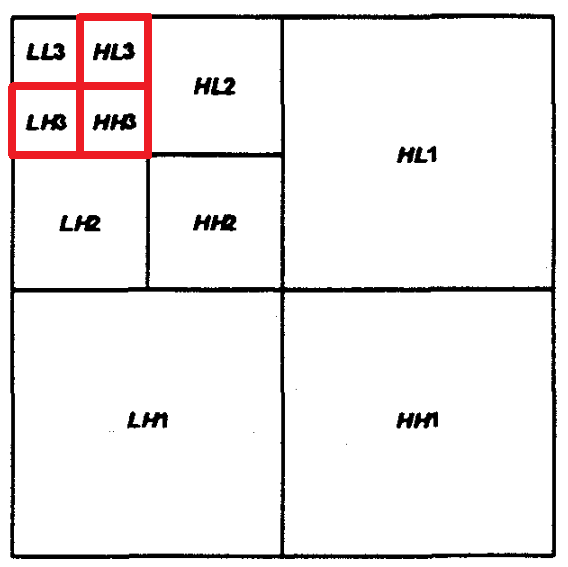
\includegraphics[width=\textwidth]{Bilder/threelayerMotivationPainted} 
	\end{figure}
	\end{minipage} 	
\end{frame}

\begin{frame}{Experimental Results}
	\begin{minipage}{0.54\textwidth}
	\begin{itemize}
	\item blind detection is used
	\item estimation of $\mu_i$ and $\sigma_i$ from watermarked image:
	\end{itemize}
$$\hat{\mu}_i = \frac{1}{N_B} \sum_{y \in B}y$$
	$$\hat{\sigma}_i = \frac{1}{N_B - 1} \sum_{y\in B}(y-\hat{\mu}_i)^2$$ 
	\end{minipage} 
	\begin{minipage}{0.44\textwidth}
	\begin{figure}
	\centering
	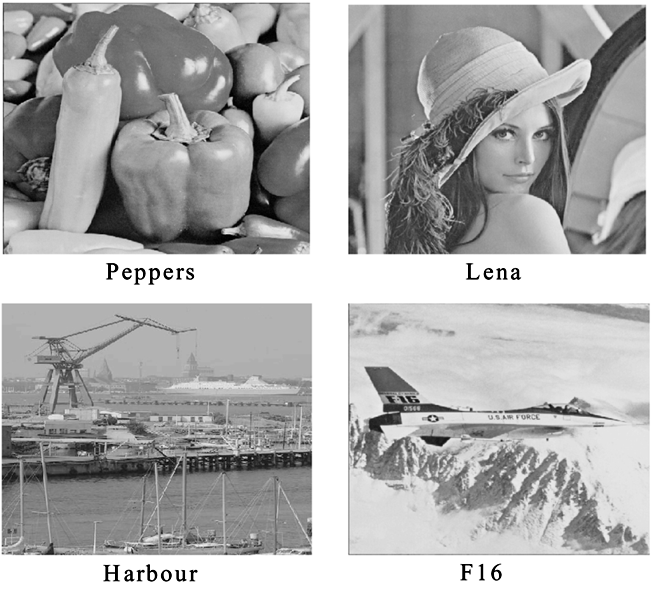
\includegraphics[width=\textwidth]{Bilder/ResultsBilder} 
	\end{figure}
	\end{minipage} 	
	with $y$ as DWT coefficient in $B$ of watermarked image
\end{frame}

%\section{Conclusion}
%\begin{frame}{\insertsection}

\textcolor{TUDblue}{Conclusion:}
\begin{itemize}
\item formulation of an ML detection scheme based on modeling the distribution of the DWT coefficients using Laplacian pdf
\item derivation of decision threshold for Neyman-Pearson criterion
\item comparison of Laplacian model with Gaussian model
\item Laplacian model yields a better watermark detection than Gaussian model
\end{itemize}

\textcolor{TUDblue}{Critique:}

\begin{itemize}
 \item $\mu_i$ and $\sigma_i$ are estimated as sample mean and unbiased sample variance 
\newline \textcolor{TUDblue}{$\Rightarrow$} inconsistent with the Laplacian assumption:
\newline $\hat{\mu}_{i, MLE} = \text{median}(y\in B)$ and $\hat{\sigma}^2_{i, MLE} = 2/N_B \sum_{y\in B} (y-\hat{\mu}_i)^2$ 

\end{itemize}
\textcolor{TUDblue}{Outlook:}
\begin{itemize}
 \item evaluation of robustness under other standard image processing operations
\end{itemize}
\end{frame}





\end{document}
